\section{Results}
Next the sparsemax transformation is evaluated using the model defined by \eqref{sparsemax-regression}. For comparison we report the softmax regression results as well. The four different implementations plus the reference softmax implementation are referred to as:
\begin{itemize}
\setlength\itemsep{-0.3em}
\item Softmax: A TensorFlow implementation of Softmax Regression.
\item Numpy: A pure Numpy implementation of Sparsemax Regression.
\item TF Numpy: A TensorFlow implementation where the custom ops associated with Sparsemax have been implemented using only Numpy.
\item TF CPU: A TensorFlow implementation where the custom ops associated with Sparsemax have been implemented in C++ for the CPU.
\item TF GPU: A TensorFlow implementation where the custom ops associated with Sparsemax have been implemented in C++ and CUDA for the GPU.
\end{itemize}
For the sake of time performance comparison all five implementations are used. For the performance only the TensorFlow C++ version of Sparsemax and Softmax are used, as the results are the same for all Sparsemax implementations.

\subsection{Label estimation}
Five well-known benchmark datasets are used, as shown in Table \ref{tab:datasets}. The digit dataset MNIST and flower dataset Iris are multi-class classification, while the Scene, Emotions and CAL500 datasets are multi-label classification.\footnote{In multi-class classification the classes are mutually exclusive, while in the multi-label case several labels can be associated with one observation reflecting a relation between the labels.} 
\begin{table}[H]
\centering
\begin{tabular}{r|cccc}
& \#Features & \#Labels & Train size & Test size \\
\hline
MNIST & 784 & 10 & 60000 & 10000 \\
Iris & 4 & 3 & 135 & 15 \\
Scene & 294 & 6 & 1211 & 1196 \\
Emotions & 72 & 6 & 391 & 202 \\
CAL500 & 68 & 174 & 451 & 51 \\
\end{tabular}

\caption{Summary for the five benchmark datasets used.}
\label{tab:datasets}
\end{table}
For comparison of performance the Jensen-Shannon divergence between the predicted and target distributions is reported.
\begin{equation*}
\mathbf{JS(q,p)}:=\frac{1}{2}\mathbf{KL}\left(\mathbf{q}\Big|\Big|\frac{\mathbf{q}+\mathbf{p}}{2}\right)+\frac{1}{2}\mathbf{KL}\left(\mathbf{p}\Big|\Big|\frac{\mathbf{q}+\mathbf{p}}{2}\right)
\end{equation*}

Where $\mathbf{p}, \mathbf{q}$ are the predicted and target distributions, respectively and $\mathbf{KL}$ is the Kullbach-Leibler distance. For all the classifiers an L2 regularizer is used and the regularization constants can be seen in Table \ref{tab:hyperparameters}. The hyperparameter was tuned using a stratified 5-split cross-validation for the MNIST and Iris datasets and non-stratified for the rest, where the resulting experiments are shown in Figure \ref{fig:hyperparameters}. The models where optimized using the Adam algorithm with default parameters, a learning rate of 0.001 and $\beta_1=0.9, \, \beta_2 = 0.999, \, \epsilon = 1\mathrm{e}{-8}$ and the Numpy implementation used Gradient Descent with a learning rate of $1\mathrm{e}{-2}$.

\begin{table}[H]
\centering
\begin{tabular}{r|ccc}
& Softmax & Sparsemax \\
\hline
MNIST & $1.00 \cdot 10^{-7}$ & $1.00 \cdot 10^{-6}$ \\
Iris & $1.00 \cdot 10^{-8}$ & $1.00 \cdot 10^{-8}$ \\
Scene & $1.00 \cdot 10^{-8}$ & $1.00 \cdot 10^{-4}$ \\
Emotions & $1.00 \cdot 10^{-8}$ & $1.00 \cdot 10^{-2}$ \\
CAL500 & $1.00 \cdot 10^{-8}$ & $1.00 \cdot 10^{-1}$ \\
\end{tabular}

\caption{Regularization values and the corresponding JS divergence for both classifiers. 5-fold cross validation was used in the training data.}
\label{tab:hyperparameters}
\end{table}
\begin{figure}[H]
	\centering
	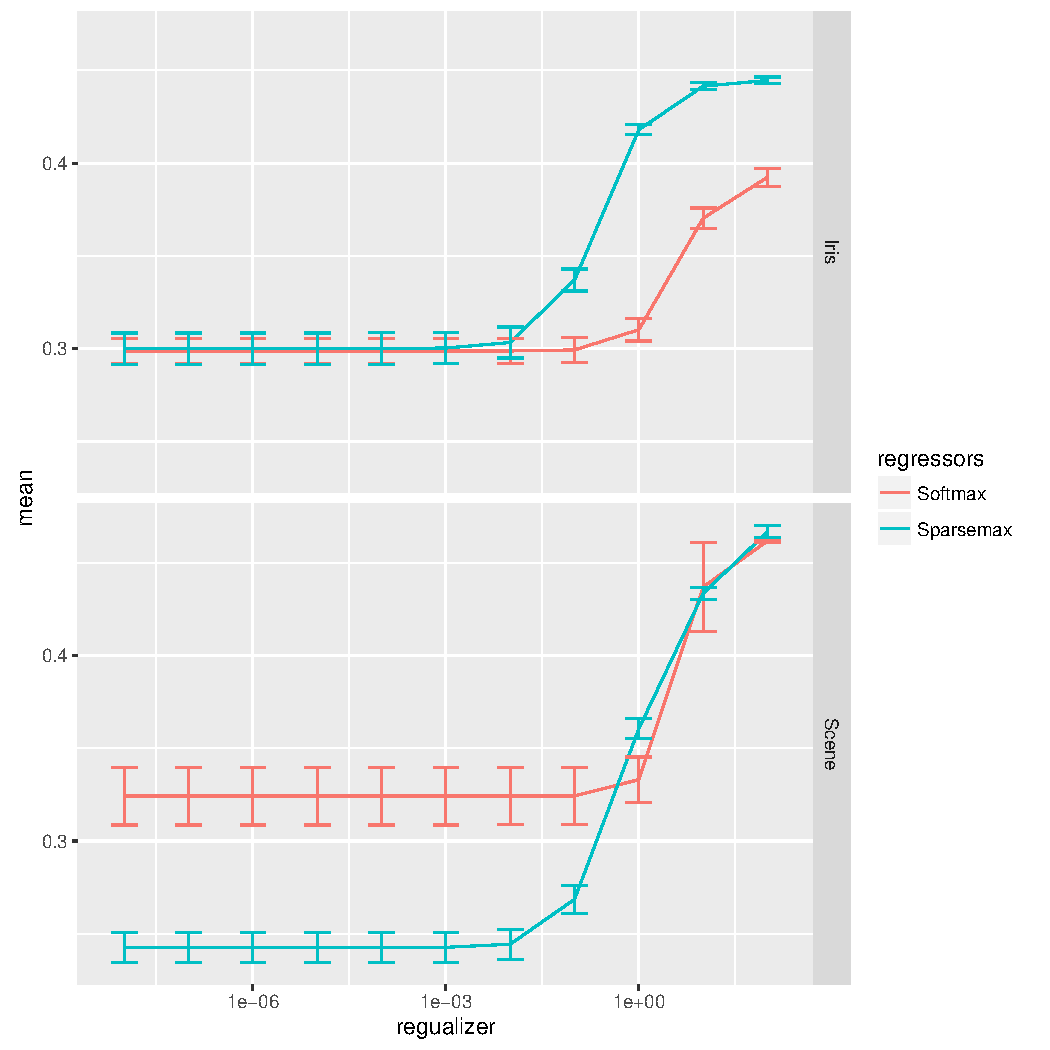
\includegraphics[scale=1]{figures/hyperparameter.pdf}
\caption{JS divergence using a range of regularizers on all five datasets for the two regressors.}
\label{fig:hyperparameters}.
\end{figure}

The JS divergence on the test set for the five datasets and the miss rate for the multi-class datasets is shown in Table \ref{tab:results}. The Softmax and Sparsemax classifier are very much alike in terms of performance. The Iris dataset shows an improved performance, comparing the two best cases in the regularization optimization (Table \ref{tab:hyperparameters}), also shows a statistical significant difference.

\begin{table}[H]
\centering
\begin{tabular}{r|ccc}
& Softmax & Sparsemax \\
\hline
MNIST & $inf \pm nan$ & $0.10 \pm 0.00$ \\
Iris & $0.15 \pm 0.00$ & $0.10 \pm 0.01$ \\
Scene & $0.30 \pm 0.01$ & $0.24 \pm 0.01$ \\
Emotions & $0.29 \pm 0.02$ & $0.27 \pm 0.02$ \\
CAL500 & $0.35 \pm 0.01$ & $0.35 \pm 0.01$ \\
\end{tabular}

\caption{JS divergence for the five benchmark datasets and the Sparsemax Classifier as well as the Softmax classifier.}
\label{tab:results}
\end{table}

\begin{table*}
\centering
\begin{tabular}{r|ccc}
& digits & iris \\
\hline
sparsemax - tensorflow numpy & $0.02 \pm 0.00$ & $0.00 \pm 0.00$ \\
sparsemax - tensorflow native & $0.01 \pm 0.00$ & $0.00 \pm 0.00$ \\
sparsemax - numpy & $0.01 \pm 0.00$ & $0.00 \pm 0.00$ \\
softmax - tensorflow & $0.02 \pm 0.00$ & $0.00 \pm 0.00$ \\
\end{tabular}

\caption{Time in seconds with associated confidence intervals.}
\label{tab:timings}
\end{table*}

\subsection{Computational performance}
The four implementations where benchmarked using the datasets from Table \ref{tab:datasets}. In Table \ref{tab:timings} the the time performance is shown and compared with the native TensorFlow Softmax implementation. Each implementation has been run for 100 epochs during timing on a Tesla K40 for the GPU implementations.

For the large dataset, MNIST, the GPU implementation significantly outperforms all other Sparsemax implementations as expected. The Numpy implementation runs significantly slower than the three TensorFlow implementations, also as expected. For the Iris dataset, which is considerably smaller in size, the Numpy and TensorFlow CPU version outperforms both the GPU and Tensorflow Numpy version. Both The TensorFlow Numpy version and the GPU version has a large overhead, which, as expected, slows the implementation. Compared to the Softmax, the GPU version of TensorFlow is significantly slower, but not by much.

\subsection{Encoder-decoder with a sparse attention mechanism}
\subsubsection{Training procedure}
Weights in the encoder-decoder model defined in \eqref{eq:attention-model} have all been initialized using a truncated random normal with a standard deviation of 0.1 except for bias terms which have been initialized using a constant initializer of 1. 

The model was optimized using the ADAM optimizer with a learning rate of 0.005, $\beta_1=0.9, \, \beta_2 = 0.999, \, \epsilon = 1\mathrm{e}{-8}$, batch sizes of 100 observations and for a 1000 epochs.

The difference in attention distribution and realized model accuracy between the attention functions can be seen in figures \ref{fig:sparsemax} and \ref{fig:softmax}.
\begin{figure}[H]
	\centering
	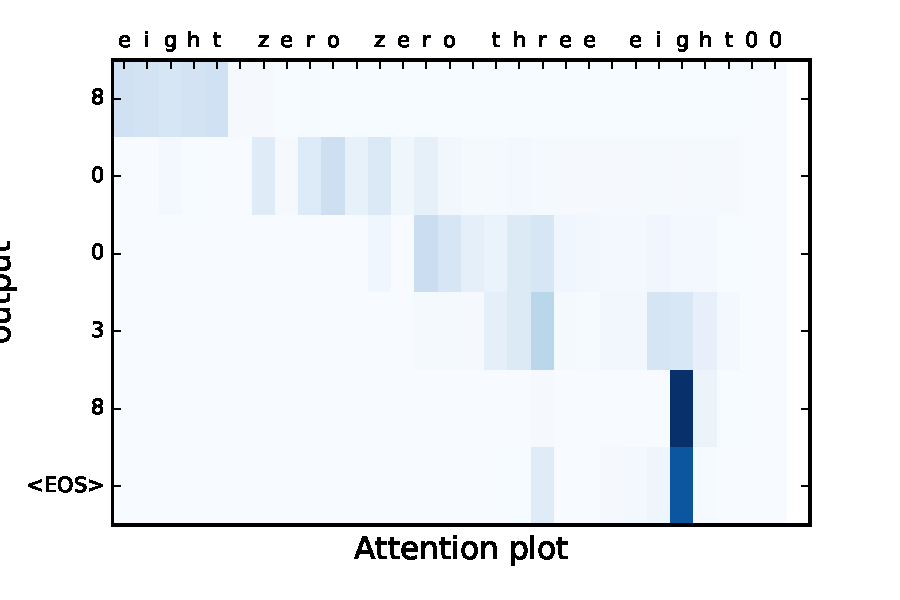
\includegraphics[scale=0.5]{figures/attention_softmax.pdf}
	\caption{Softmax attention for an Encoder-Decoder RNN. Validation accuracy after 100k training examples: $\approx 75$\%.}
	\label{fig:softmax}.
\end{figure}
\begin{figure}[H]
 	\centering
 	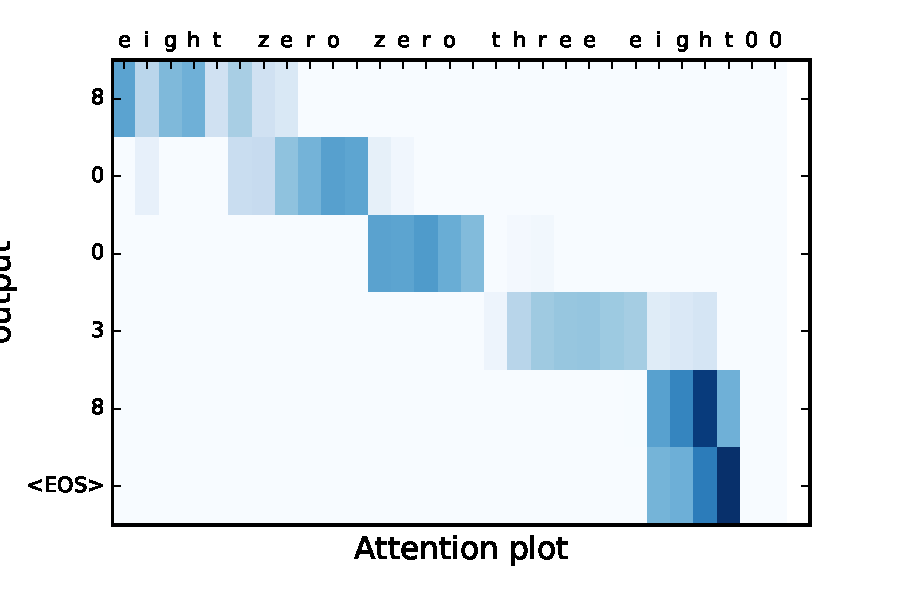
\includegraphics[scale=0.5]{figures/attention_sparsemax.pdf}
 	\caption{Sparsemax attention for an Encoder-Decoder RNN. Validation accuracy after 100k training examples: $\approx 98$\%.}
 	\label{fig:sparsemax}.
\end{figure}
  
